\begin{figure}[H]
    \centering
    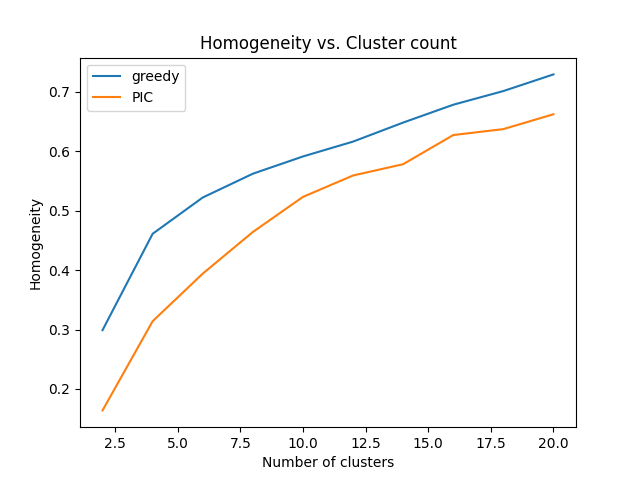
\includegraphics[width=0.45\textwidth]{assets/results/dbpediaProfiles/homogenity_comparison.png}
    \caption{Homogeneity vs Number of clusters for dbpediaProfiles data set}
    \label{fig:homogenity_dbpediaProfiles}
\end{figure}

\begin{figure}[H]
    \centering
    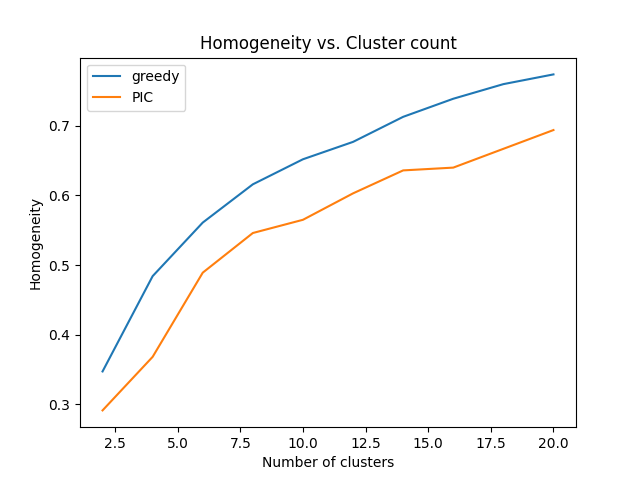
\includegraphics[width=0.45\textwidth]{assets/results/dunkin_stores/homogenity_comparison.png}
    \caption{Homogeneity vs Number of clusters for Dunkin stores data set}
    \label{fig:homogenity_dunkin_stores}
\end{figure}

\begin{figure}[H]
    \centering
    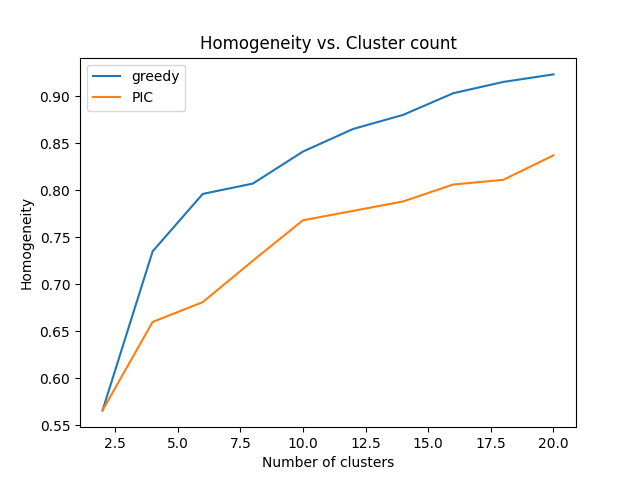
\includegraphics[width=0.45\textwidth]{assets/results/syntheticFincances/homogenity_comparison.png}
    \caption{Homogeneity vs Number of clusters for synthetic Finance data set}
    \label{fig:homogenity_syntheticFinance}
\end{figure}

\begin{figure}[H]
    \centering
    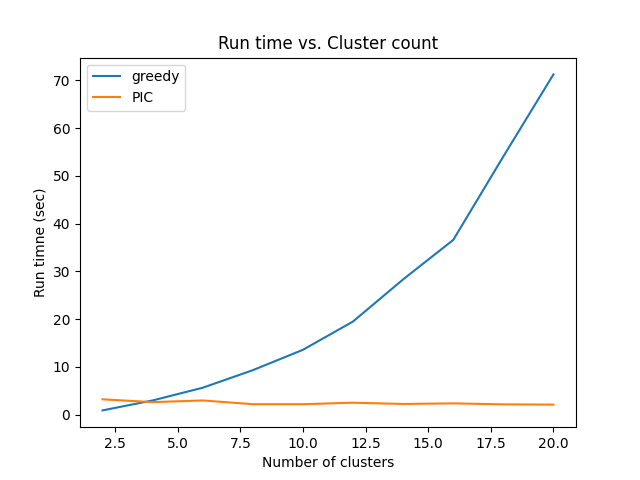
\includegraphics[width=0.45\textwidth]{assets/results/dbpediaProfiles/run_time_comparison.png}
    \caption{Run time vs Number of clusters for dbpediaProfiles data set}
    \label{fig:runtime_dbpediaProfiles}
\end{figure}

\begin{figure}[H]
    \centering
    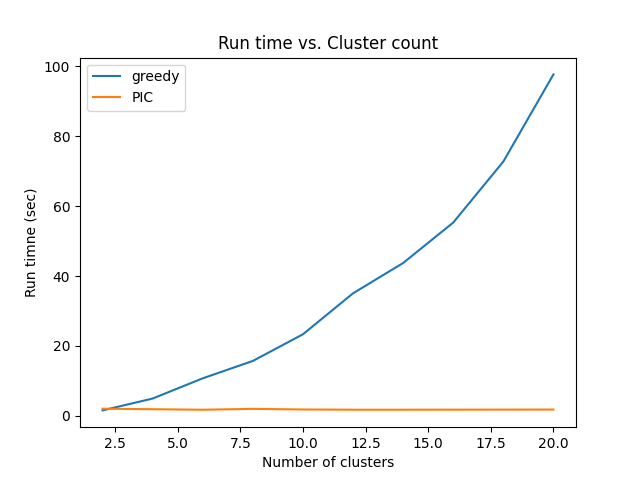
\includegraphics[width=0.45\textwidth]{assets/results/dunkin_stores/run_time_comparison.png}
    \caption{Run time vs Number of clusters for Dunkin stores data set}
    \label{fig:runtime_dunkin_stores}
\end{figure}

\begin{figure}[H]
    \centering
    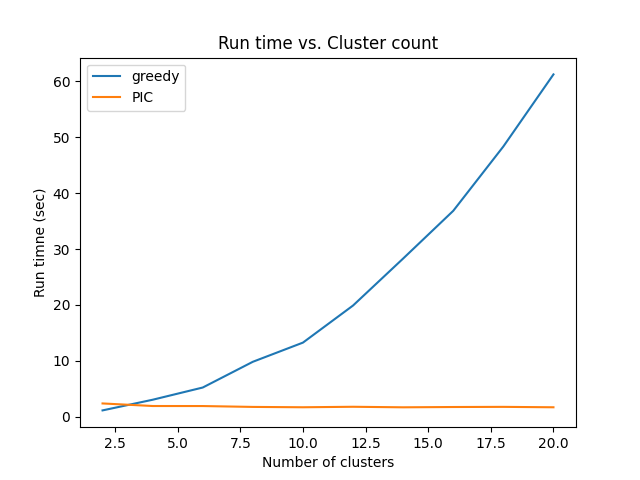
\includegraphics[width=0.45\textwidth]{assets/results/syntheticFincances/run_time_comparison.png}
    \caption{Run time vs Number of clusters for synthetic Finance stores data set}
    \label{fig:runtime_syntheticFinance}
\end{figure}

\clearpage

\begin{figure}
    \centering
    \resizebox{0.95\textwidth}{!}{\begin{tabular}[c]{cc}
    \begin{subfigure}[c]{0.45\textwidth}
         \centering
         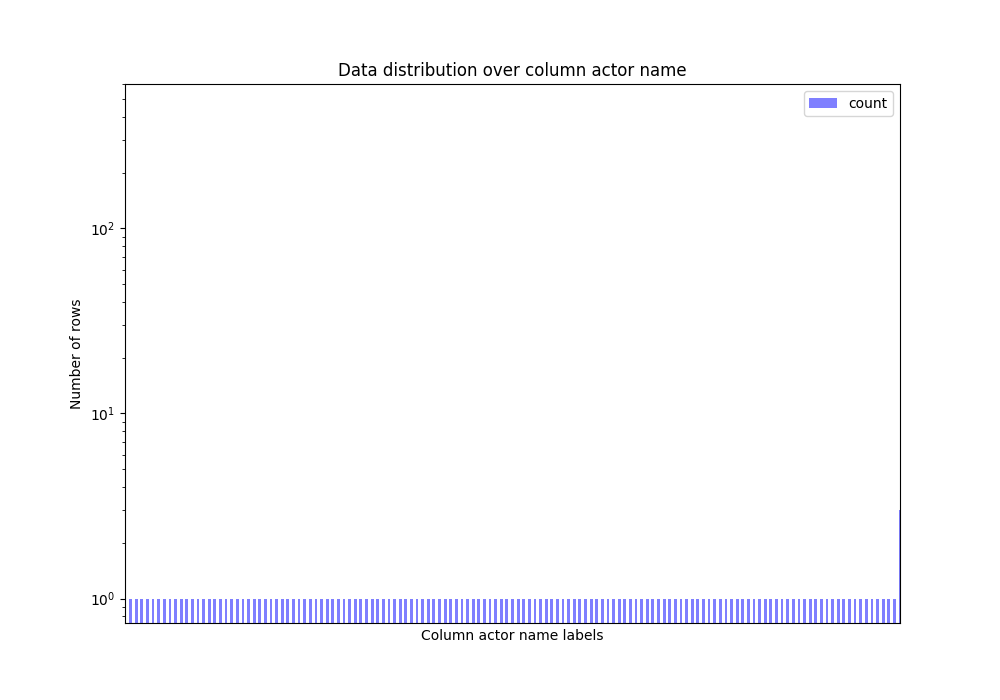
\includegraphics[width=\textwidth]{assets/results/dbpediaProfiles/distribution/actor name.png}
         \caption{Actor name}
         \label{}
     \end{subfigure} &
     \begin{subfigure}[c]{0.45\textwidth}
         \centering
         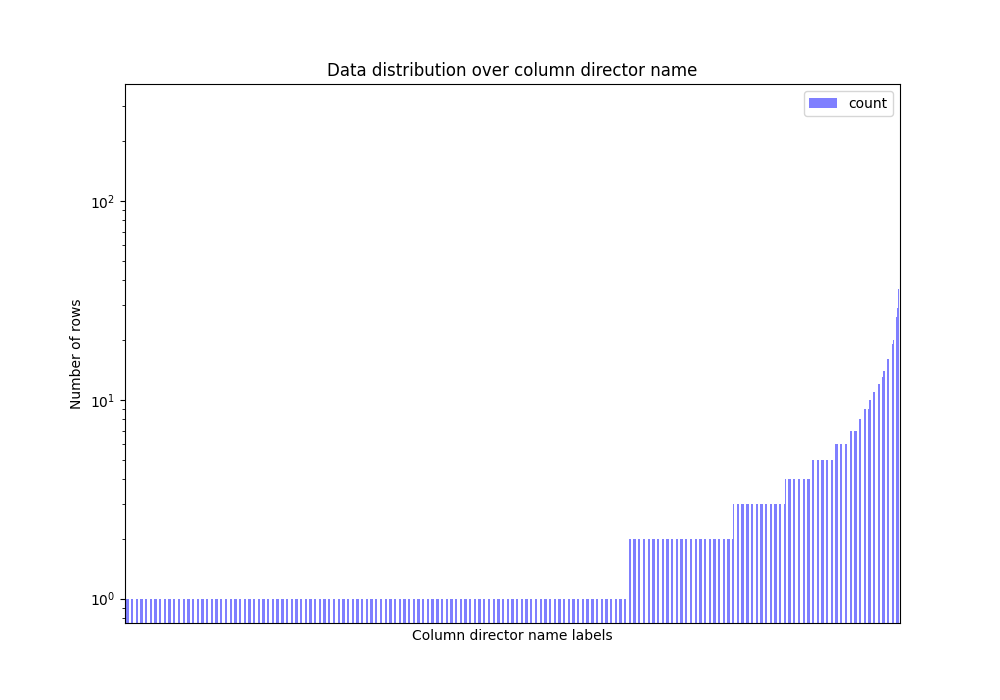
\includegraphics[width=\textwidth]{assets/results/dbpediaProfiles/distribution/director name.png}
         \caption{Director name}
         \label{}
     \end{subfigure} \\
     
     \begin{subfigure}[c]{0.45\textwidth}
         \centering
         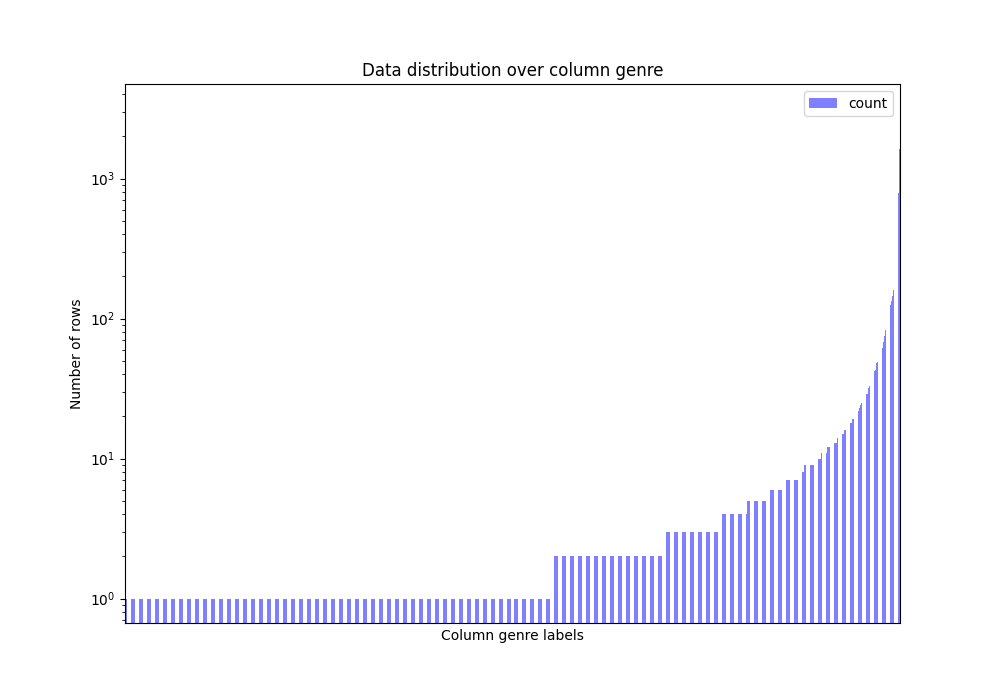
\includegraphics[width=\textwidth]{assets/results/dbpediaProfiles/distribution/genre.png}
         \caption{Genre}
         \label{}
     \end{subfigure} &
     \begin{subfigure}[c]{0.45\textwidth}
         \centering
         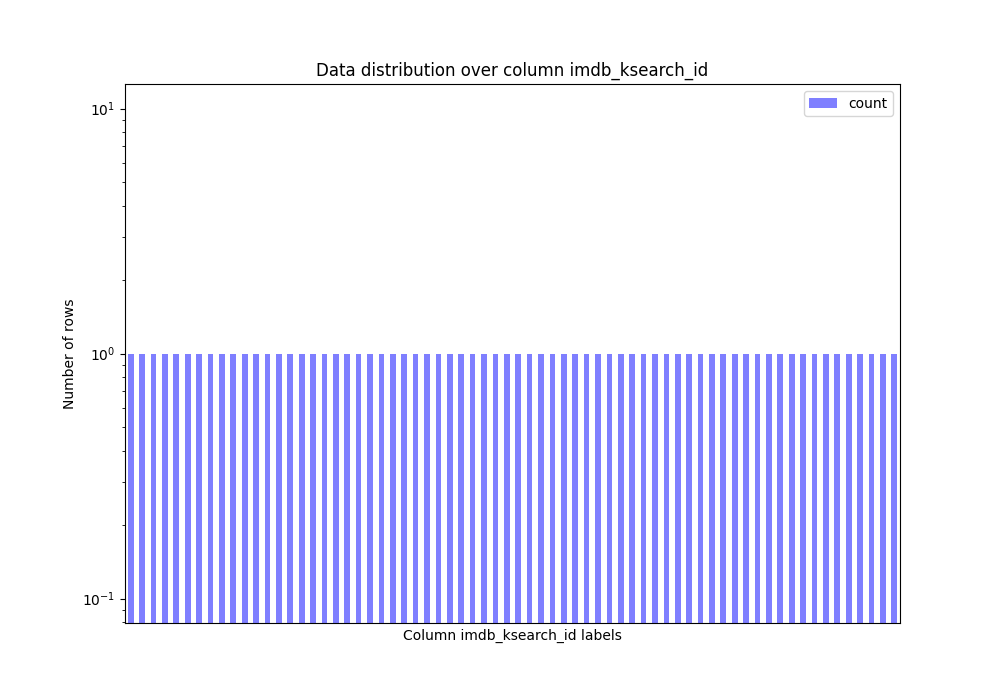
\includegraphics[width=\textwidth]{assets/results/dbpediaProfiles/distribution/imdb_ksearch_id.png}
         \caption{Imdb ksearch id}
         \label{}
     \end{subfigure} \\
     \begin{subfigure}[c]{0.45\textwidth}
         \centering
         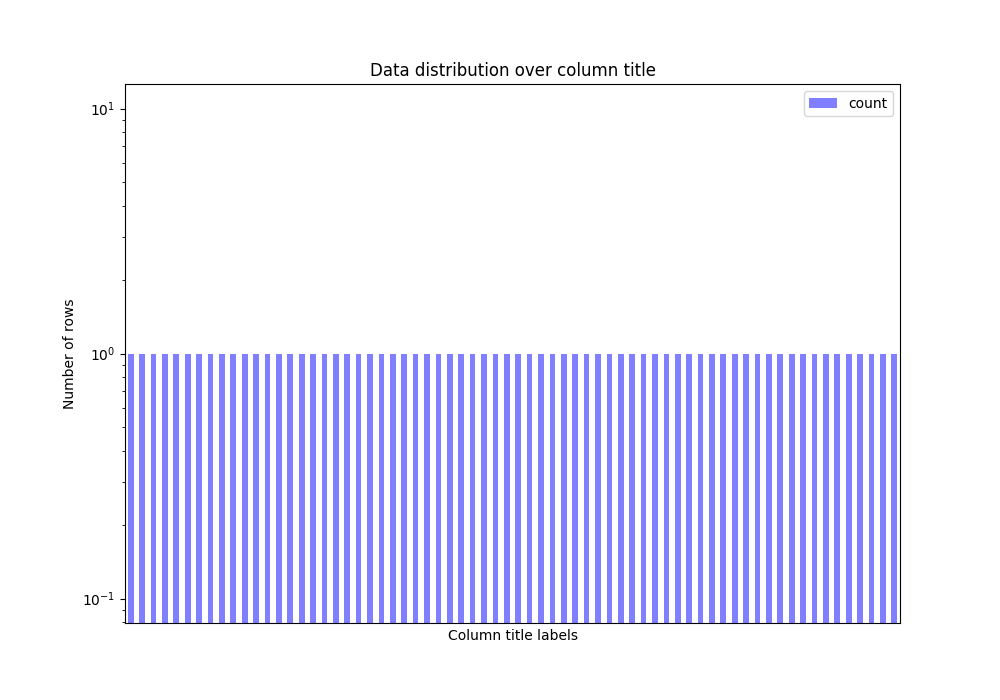
\includegraphics[width=\textwidth]{assets/results/dbpediaProfiles/distribution/title.png}
         \caption{Title}
         \label{}
     \end{subfigure} &
     \begin{subfigure}[c]{0.45\textwidth}
         \centering
         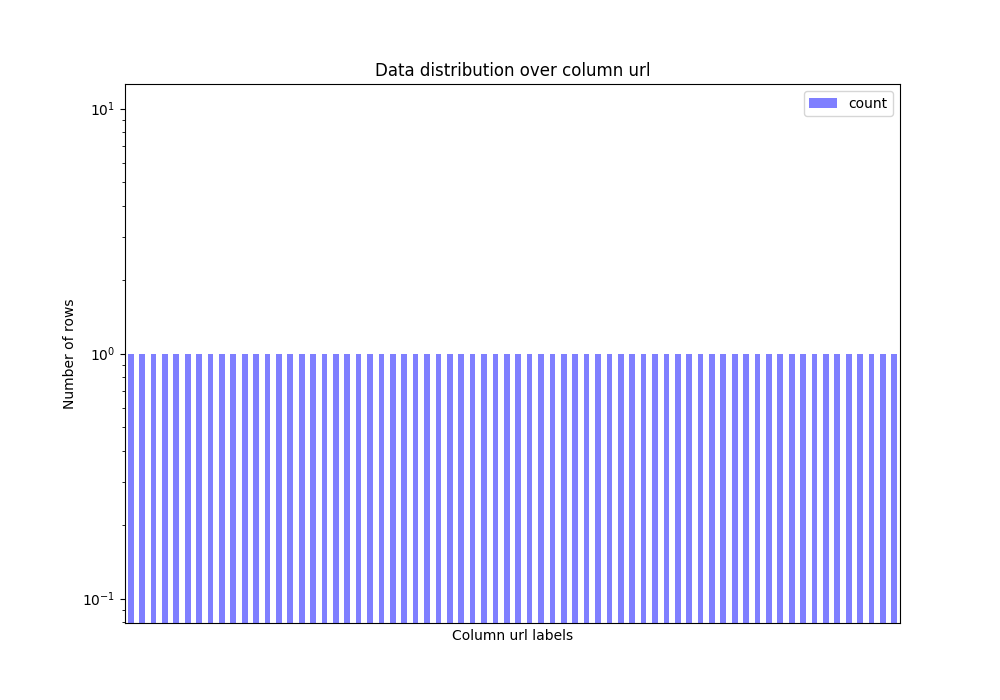
\includegraphics[width=\textwidth]{assets/results/dbpediaProfiles/distribution/url.png}
         \caption{Url}
         \label{}
     \end{subfigure} \\
     \multicolumn{2}{c}{\begin{subfigure}[c]{0.45\textwidth}
         \centering
         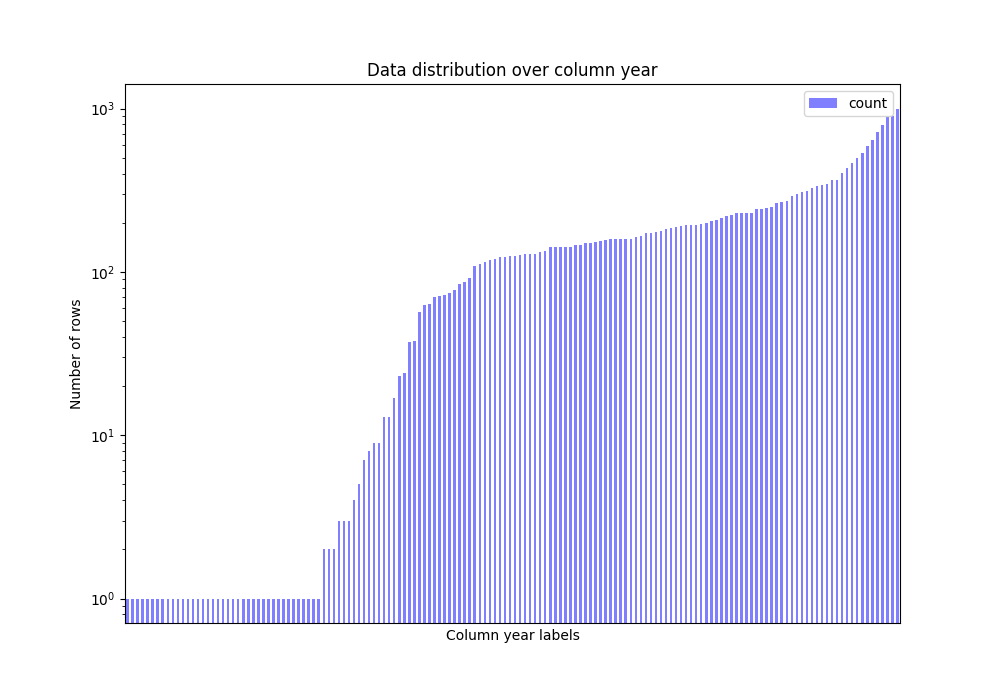
\includegraphics[width=\textwidth]{assets/results/dbpediaProfiles/distribution/year.png}
         \caption{Year}
         \label{}
     \end{subfigure}}
     \end{tabular}
     }
    \caption{Distribution analysis for dbpediaProfiles data set}
    \label{fig:dbpediaProfiles_distribution_analysis}
\end{figure}

\clearpage

\begin{figure}
    \centering
    \resizebox{0.7\textwidth}{!}{\begin{tabular}[c]{cc}
    \begin{subfigure}[c]{0.45\textwidth}
         \centering
         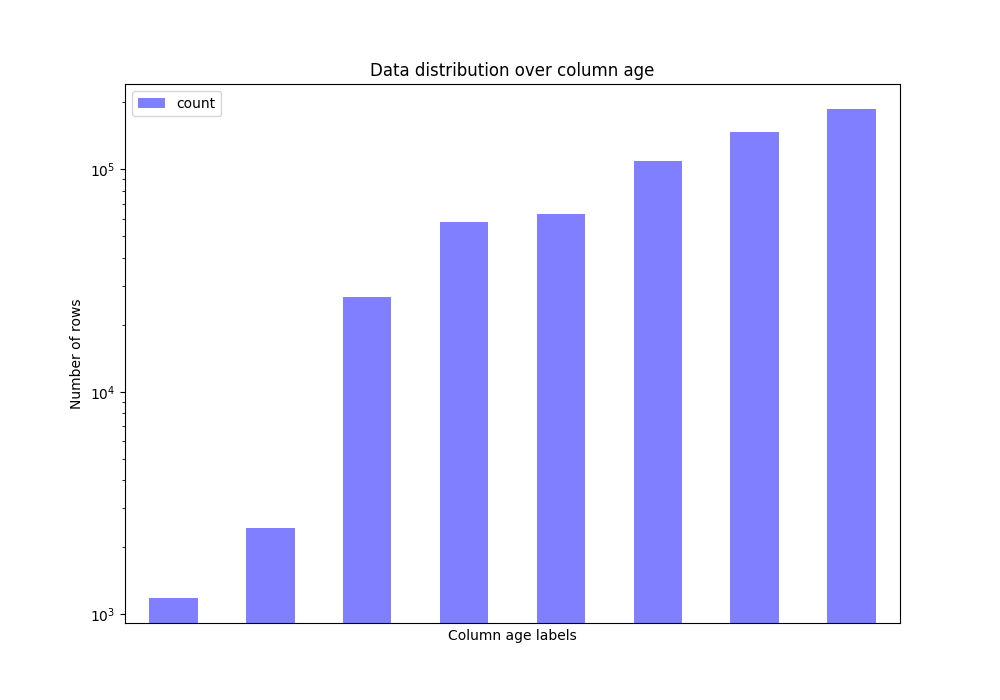
\includegraphics[width=\textwidth]{assets/results/syntheticFincances/distribution/age.png}
         \caption{Age}
         \label{}
     \end{subfigure} &
     
     \begin{subfigure}[c]{0.45\textwidth}
         \centering
         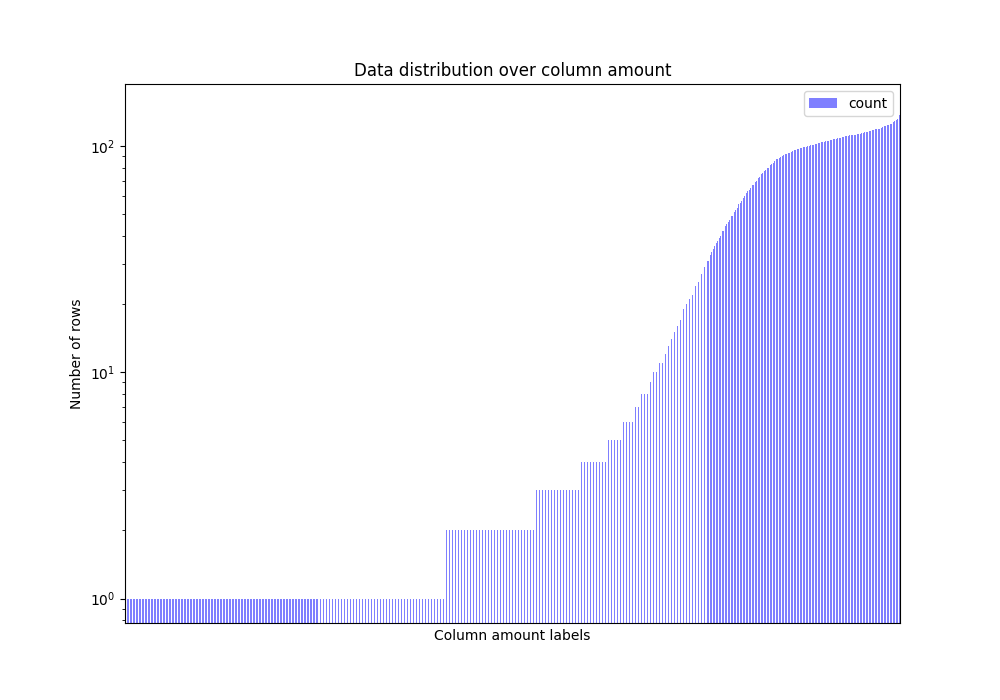
\includegraphics[width=\textwidth]{assets/results/syntheticFincances/distribution/amount.png}
         \caption{Amount}
         \label{}
     \end{subfigure} \\
     
     \begin{subfigure}[c]{0.45\textwidth}
         \centering
         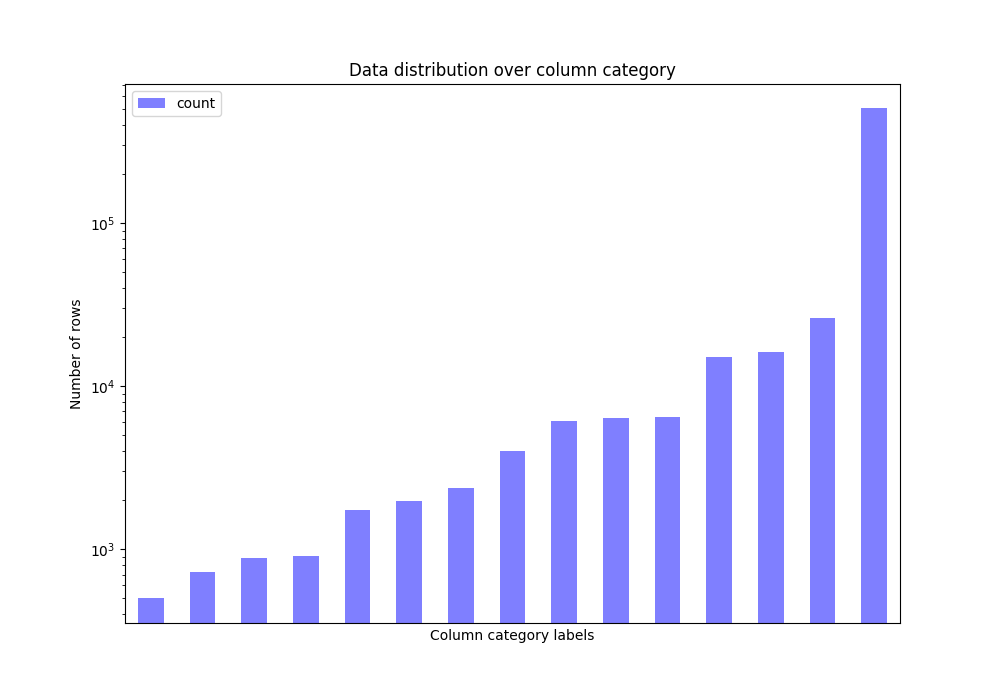
\includegraphics[width=\textwidth]{assets/results/syntheticFincances/distribution/category.png}
         \caption{Category}
         \label{}
     \end{subfigure} &
     
     \begin{subfigure}[c]{0.45\textwidth}
         \centering
         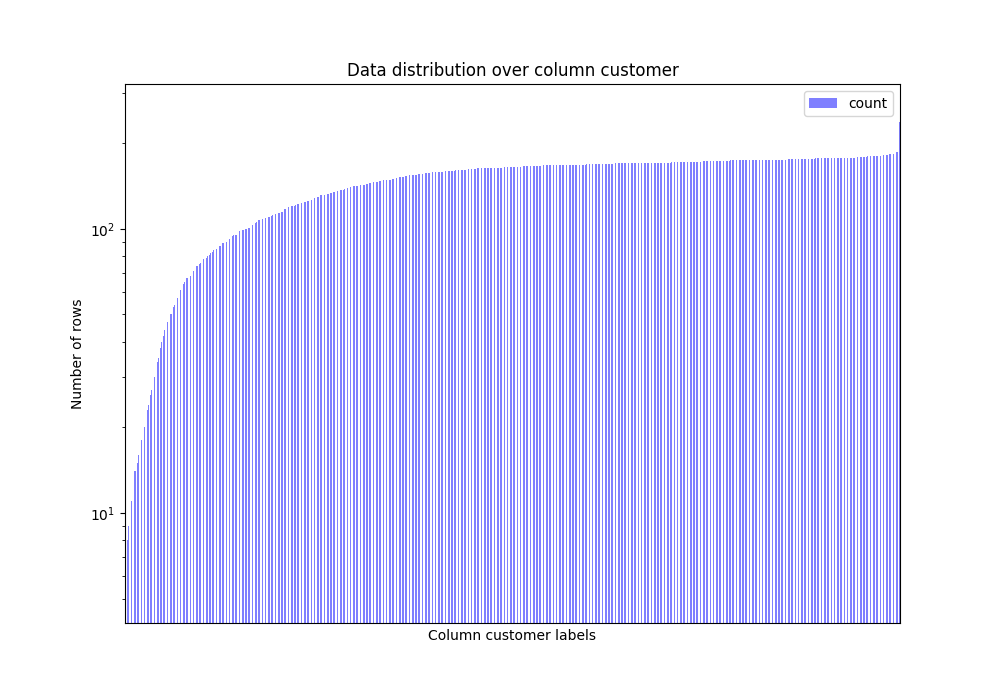
\includegraphics[width=\textwidth]{assets/results/syntheticFincances/distribution/customer.png}
         \caption{Customer}
         \label{}
     \end{subfigure} \\
     
     \begin{subfigure}[c]{0.45\textwidth}
         \centering
         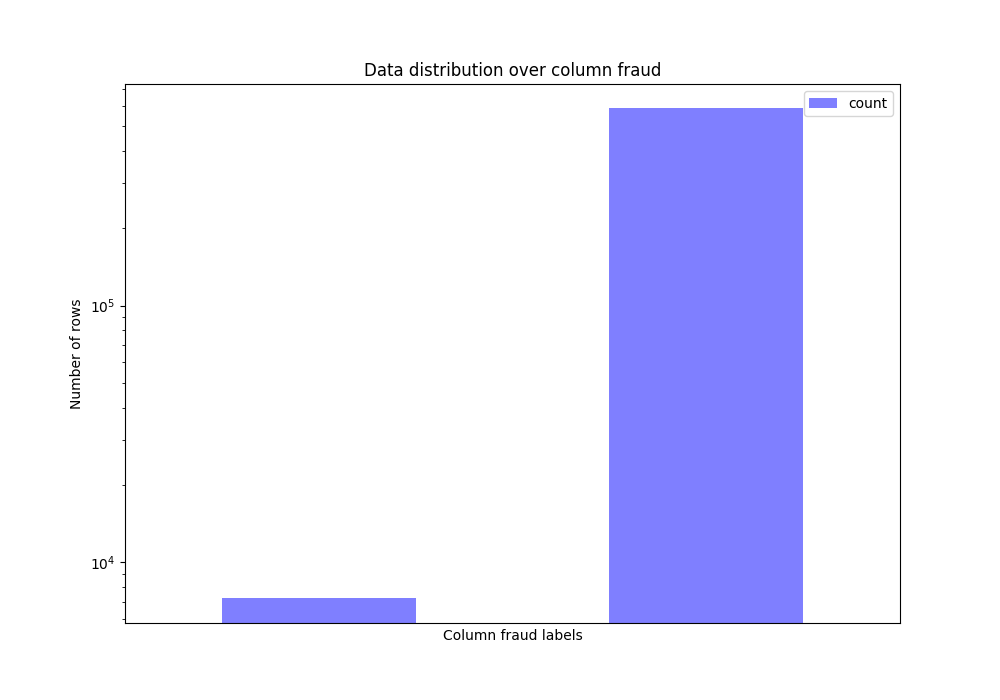
\includegraphics[width=\textwidth]{assets/results/syntheticFincances/distribution/fraud.png}
         \caption{Fraud}
         \label{}
     \end{subfigure} &
     
     \begin{subfigure}[c]{0.45\textwidth}
         \centering
         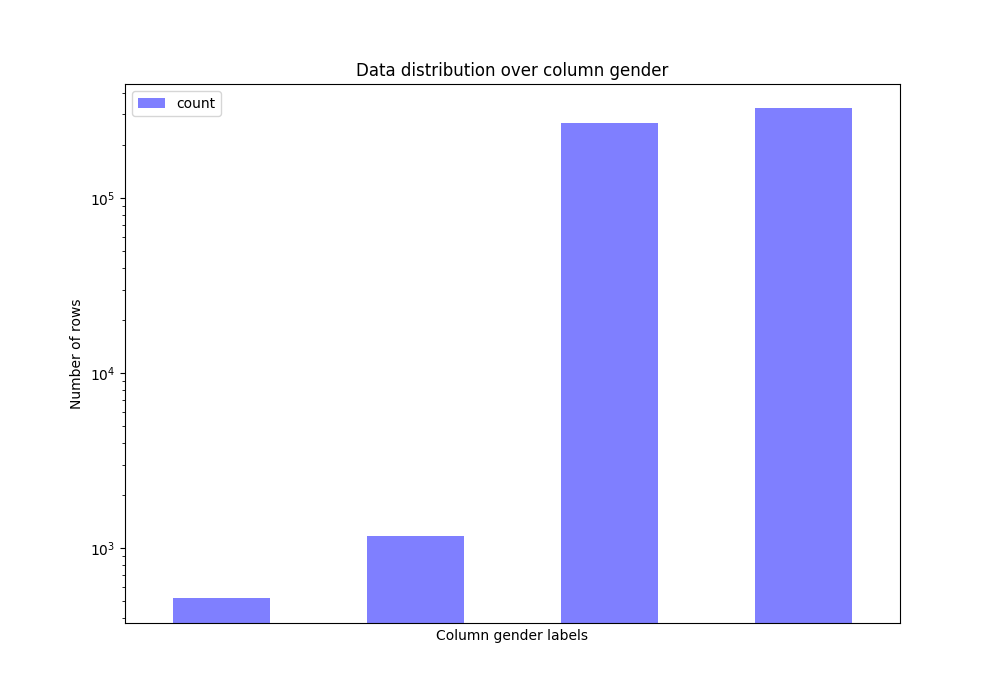
\includegraphics[width=\textwidth]{assets/results/syntheticFincances/distribution/gender.png}
         \caption{Gender}
         \label{}
     \end{subfigure}  \\
     
     \begin{subfigure}[c]{0.45\textwidth}
         \centering
         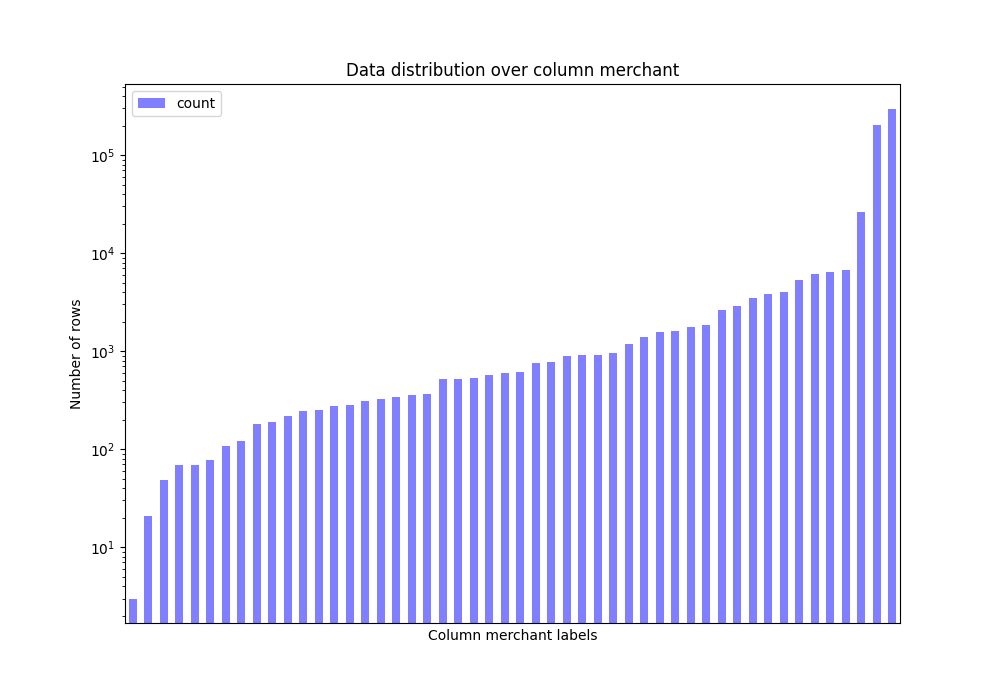
\includegraphics[width=\textwidth]{assets/results/syntheticFincances/distribution/merchant.png}
         \caption{Merchant}
         \label{}
     \end{subfigure} &
     
     \begin{subfigure}[c]{0.45\textwidth}
         \centering
         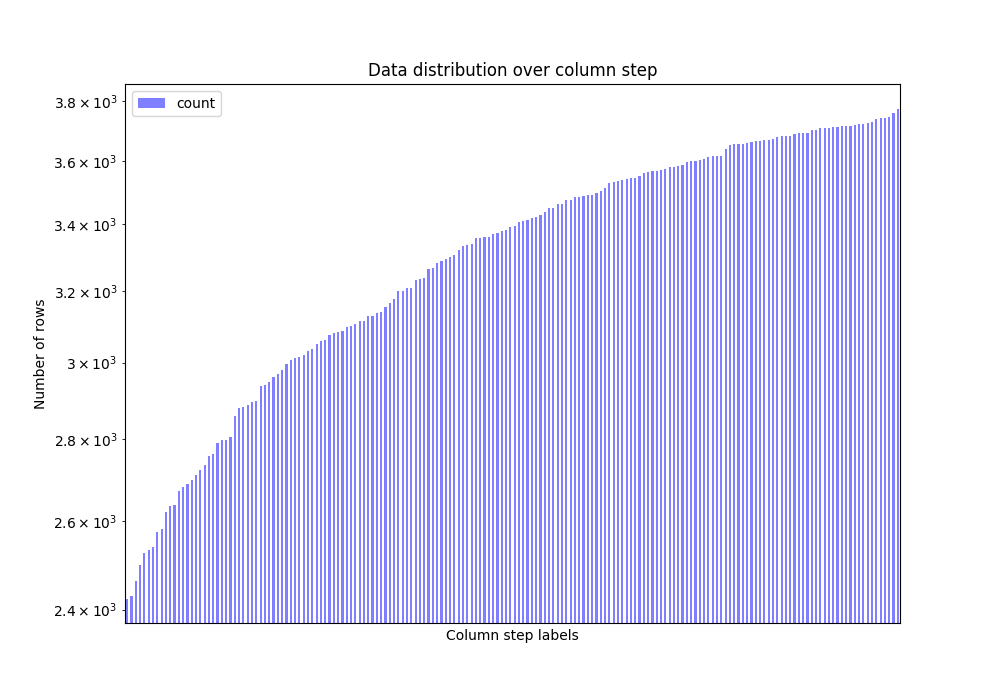
\includegraphics[width=\textwidth]{assets/results/syntheticFincances/distribution/step.png}
         \caption{Step}
         \label{}
     \end{subfigure} \\
     
     \begin{subfigure}[c]{0.45\textwidth}
         \centering
         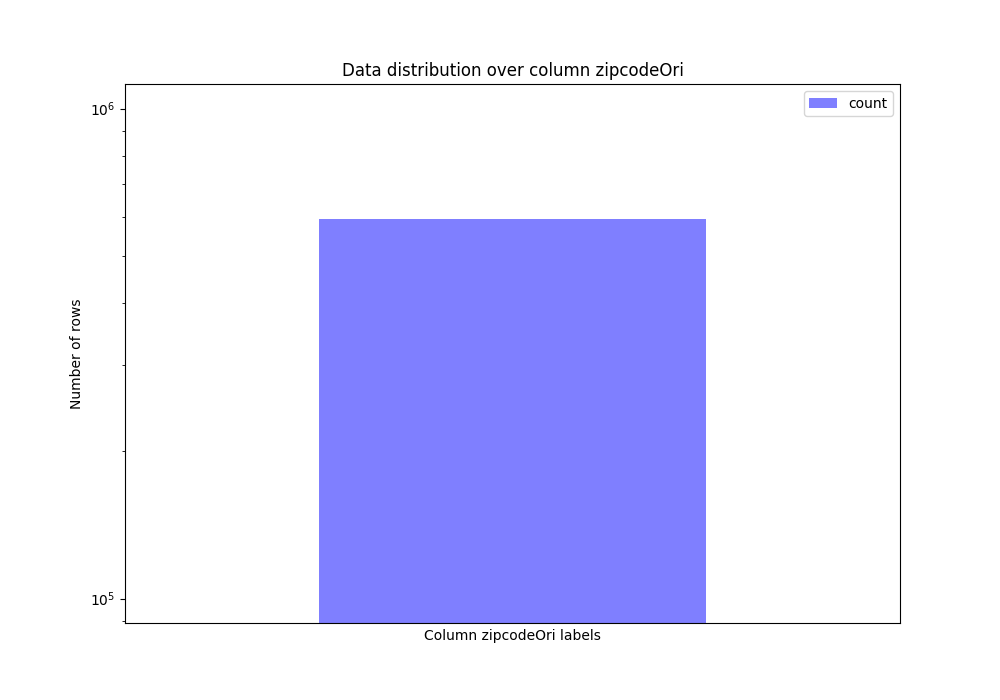
\includegraphics[width=\textwidth]{assets/results/syntheticFincances/distribution/zipcodeOri.png}
         \caption{zipcodeOri}
         \label{}
     \end{subfigure} &
     
     \begin{subfigure}[c]{0.45\textwidth}
         \centering
         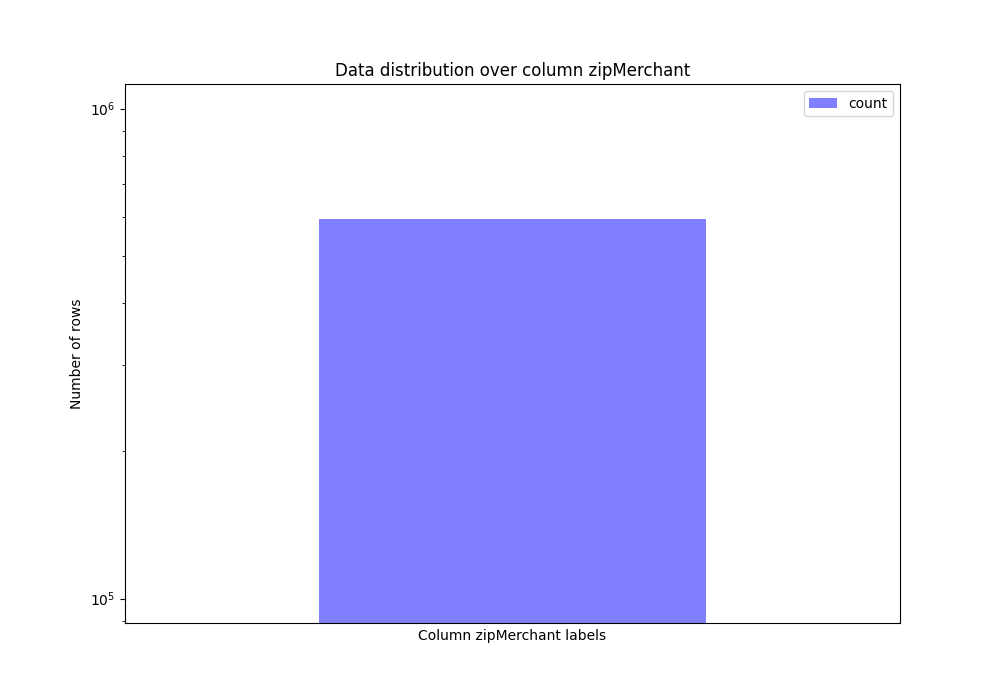
\includegraphics[width=\textwidth]{assets/results/syntheticFincances/distribution/zipMerchant.png}
         \caption{zipMerchant}
         \label{}
     \end{subfigure} 
     \end{tabular} 
     }
    \caption{Distribution analysis for synthetic Finance}
    \label{fig:synthetic_finance_distribution_analysis}
\end{figure}